\documentclass[xcolor=table]{beamer}
\usetheme{Madrid}
\usepackage{amssymb}
\usepackage{epsfig}
\usepackage{psfrag}
\usepackage{wrapfig}
\usepackage{graphicx}
\usepackage{color}
\usepackage{amsmath}
\usepackage{multimedia}
%\usepackage{style}
\usepackage{verbatim}
\usepackage{listings}
\usepackage{multicol}
\usepackage[table]{xcolor}

\DeclareSymbolFont{nosets}{U}{msb}{m}{7}
\DeclareMathSymbol{\natural}{\mathalpha}{nosets}{'116} %can be done with \Bbb see page 218
\DeclareMathSymbol{\real}{\mathalpha}{nosets}{'122}
\DeclareMathSymbol{\complex}{\mathalpha}{nosets}{'103}
\DeclareMathSymbol{\integer}{\mathalpha}{nosets}{'132}
\newcommand{\cross}{\wedge}
\newcommand{\vecdiv}{\nabla \cdot}
\newcommand{\grad}{\nabla}
\newcommand{\curl}{\nabla \cross}
\newcommand{\ifff}{\Leftrightarrow} % \iff is already used
\newcommand{\sgn}{\text{sgn}}
\newcommand{\vect}[1]{\mathbf{#1}}
\newcommand{\sectref}[1]{\S\ref{#1}}
\providecommand{\norm}[1]{\lVert#1\rVert}
\numberwithin{equation}{section}
\usefonttheme{professionalfonts}
%\usefonttheme[stillsansseriflarge,stillsansserifsmall]{serif}

% BA defined commands
\let\bs\boldsymbol
\DeclareMathOperator*{\argmin}{arg\,min}
%
\lstset{language=C++}
\lstset{otherkeywords={<<<,>>>}}
\lstset{morekeywords={dim3,__host__,__kernel__,__global__,__device__}}
\lstset{breaklines,breakatwhitespace,breakautoindent=false,showstringspaces=false}
\lstset{keywordstyle=\color{purple}}
\lstset{identifierstyle=\color{blue}}
\lstset{basicstyle=\fontfamily{pcr}\fontsize{9pt}{9pt}\selectfont}
%\lstset{numbers=left, numberstyle=\tiny, stepnumber=1, numbersep=5pt}
\lstset{linewidth=4.9in,xleftmargin=10pt}

\definecolor{lightblue}{rgb}{0.0,0.45,0.81}
\definecolor{lighterblue}{rgb}{0.415,0.678,0.894}
\definecolor{darkblue}{rgb}{0,0.243,0.447}
\setbeamercolor{frametitle}{bg=lightblue,fg=white}
\setbeamerfont{normal text}{family=helvet}
\setbeamerfont{local structure}{family=helvet}

\setbeamercolor*{author in head/foot}{bg=darkblue}
\setbeamercolor*{logo in head/foot}{bg=darkblue,fg=white}
\setbeamercolor*{title in head/foot}{bg=darkblue,fg=white}
\setbeamercolor*{date in head/foot}{bg=darkblue,fg=white}
\setbeamercolor{title}{bg=darkblue}
\setbeamercolor{under headline}{bg=lighterblue}
\setbeamercolor{footline}{bg=darkblue}

\setbeamerfont*{title in head/foot}{size=\small}
\setbeamerfont*{date in head/foot}{size=\small}


\setbeamertemplate{frametitle}
{
  \leavevmode%
  \begin{beamercolorbox}[wd=\paperwidth,ht=1cm]{frametitle}
   \hspace{1em}\insertframetitle\vspace{0.35cm}
   \end{beamercolorbox}%
   \vskip-0.4cm%
  \begin{beamercolorbox}[wd=\paperwidth,ht=1ex]{under headline}%
    \end{beamercolorbox}%
	
}

%\setbeamerfont{frametitle}{series=\bfseries}
\setbeamertemplate{footline}
{
  \leavevmode%
  \hbox{%
  \begin{beamercolorbox}[wd=.3\paperwidth,ht=0.8cm,center,dp=1ex]{logo in
    head/foot}%
  \usebeamerfont{logo in head/foot}
\includegraphics[width=.25\paperwidth]{./UClogo_bg.png}%
\end{beamercolorbox}%
  \begin{beamercolorbox}[wd=.28\paperwidth,center,dp=1ex,ht=0.8cm]{title in head/foot}%
    \usebeamerfont{title in head/foot}Machine Learning \& Compressive Sensing\vspace{0.05cm}
  \end{beamercolorbox}%
  \begin{beamercolorbox}[wd=.35\paperwidth,dp=1ex,center,ht=0.8cm]{date in head/foot}%
    \usebeamerfont{date in head/foot}Laboratory for Scientific
    Computing\vspace{0.05cm}
\end{beamercolorbox}%
\begin{beamercolorbox}[wd=0.07\paperwidth,ht=0.8cm,dp=1ex,right,topskip=1em]{date
    in head/foot}%
    \insertframenumber{} / \inserttotalframenumber\hspace*{2ex}\vspace{0.3cm}
  \end{beamercolorbox}}%
  \vskip0pt%
}



\title[Beamer Intro]{Compressive Sensing in Video Encoding}
\author{Brian Azizi}
\institute[LSC]{Laboratory for Scientific Computing, University of Cambridge}
\date{\today}
\begin{document}
\begin{frame}
  \titlepage
  \begin{tabbing}
    Thanks to:  \= Dr Anita Faul (Supervisor)\\
    \>Dr Nikos Nikiforakis\\
    \>Georgios Pilikos
  \end{tabbing}
\end{frame}

\begin{frame}{Outline}
\begin{itemize}
\item Project Outcome \& Demonstration
\item Theoretical Background
\item Further Work 
\item More demos of results
\item Bibliography
\end{itemize}
\end{frame}

\begin{frame}{2D Demonstration}
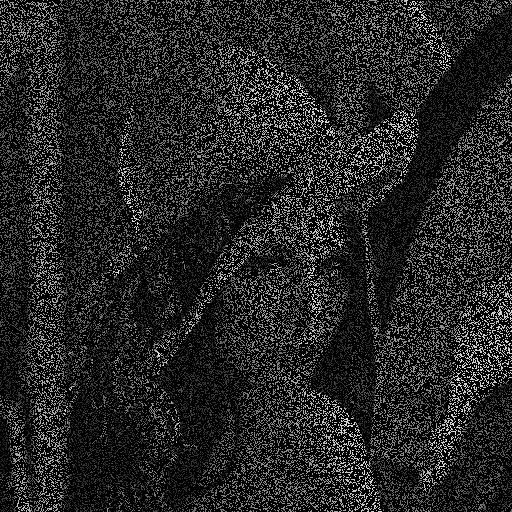
\includegraphics[width=2in,height=2in]{L0.png}
\hspace{0.2in}
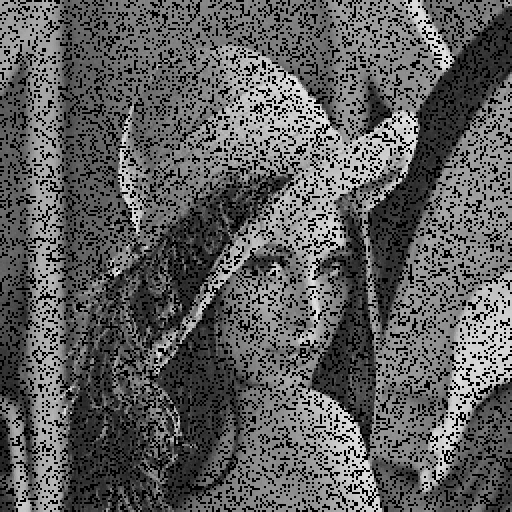
\includegraphics[width=2in,height=2in]{L1.png}\\
\hspace{0in} Corrupted Image (70\% missing) \hspace{0.5in} Scale 1 Reconstruction\\
\vspace{0.2in}
See 2014 MPhil Thesis by Georgios Pilikos
\end{frame}

\begin{frame}{2D Demonstration}
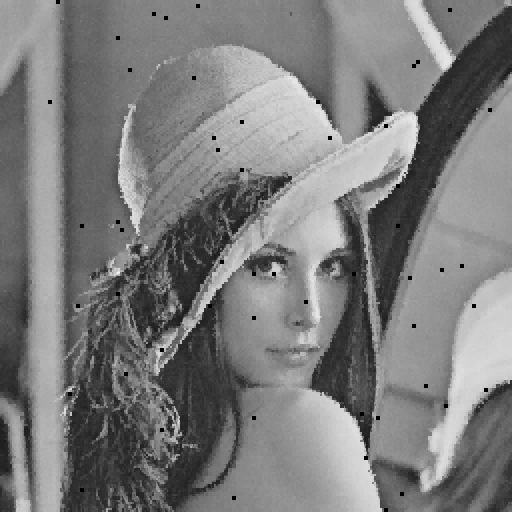
\includegraphics[width=2in,height=2in]{L2.png}
\hspace{0.2in}
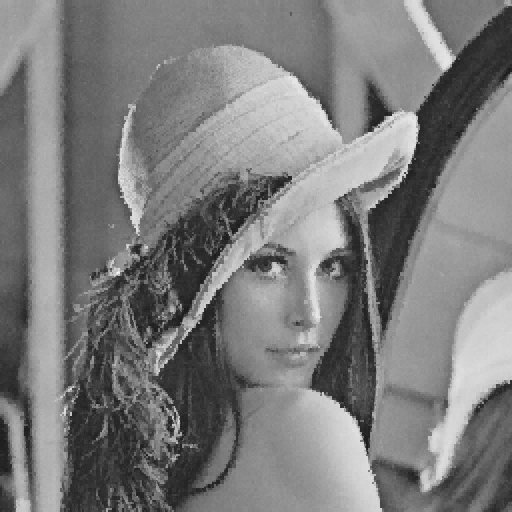
\includegraphics[width=2in,height=2in]{L3.png}\\
\hspace{0.4in} Cascade to scale 2 \hspace{1in} Cascade to scale 3\\
\vspace{0.2in}
See 2014 MPhil Thesis by Georgios Pilikos
\end{frame}

\begin{frame}{3D Demonstration}
\hspace{1.8in}Current prototype:\\
\movie{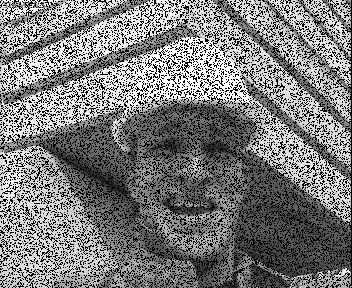
\includegraphics[height=1.8in,width=2.2in]{foreman_corr.png}}{foreman_corr.avi}
\,
\movie{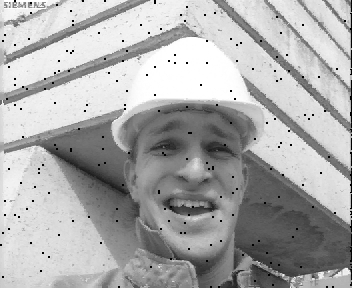
\includegraphics[height=1.8in,width=2.2in]{foreman_rec.png}}{foreman_rec.avi}\\
\hspace{0.1in} Corrupted Video (60\% missing) \hspace{0.5in} Scale 1 Reconstruction \\
\end{frame}

\begin{frame}{3D Demonstration}
\begin{itemize}
\item No cascade of reconstructions yet - ask me later this week
\item For reference, the original video:
\end{itemize}
\hspace{1in}
\movie{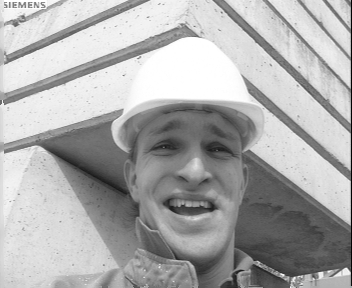
\includegraphics[height=1.8in,width=2.2in]{foreman_raw.png}}{foreman_raw.avi}
\end{frame}

\begin{frame}{Theoretical Background}
\begin{itemize} %[<+->]
\item Three building blocks:
\begin{itemize}
\item \emph{Compressive Sensing} - Novel signal processing framework allowing for near-perfect reconstruction of heavily under-sampled signals
\item \emph{Discrete Wavelet Transforms} - Required for obtaining sparse representations of the signals
\item \emph{Relevance Vector Machine} - Machine Learning Algorithm for performing the reconstruction via regression
\end{itemize}
\end{itemize}
\end{frame}

\begin{frame}{Compressive Sensing: Reconstruction}
\begin{itemize}%[<+->]
\item General idea: Reconstruct signal $\bs x\in\mathbb{R}^N$ from measurements $\bs y\in\mathbb{R}^M$ where $M<<N$
\item Corresponds to solving under-determined linear system $\Omega \bs x = \bs y$, $\Omega \in \mathbb{R}^{M\times N}$
\item In general, shouldn't be possible by fundamental theorem of Linear Algebra (``as many equations as unknowns'')
\end{itemize}
\end{frame}

\begin{frame}{Compressive Sensing: Reconstruction}
\begin{itemize}%[<+->]
\item However, for a certain class of signals it is possible to get perfect reconstruction. Namely if
\begin{enumerate}
\item $\bs x$ is \emph{sparse} (i.e. most elements are zero), or
\item it is possible to change basis so that the transformed signal $\bs w = \Psi^T \bs x$ is sparse
\end{enumerate}
\item So in the later case: $\bs y = \Omega\bs x = \Omega\Psi \bs w \equiv \Phi\bs w$
\item We know $\bs y \in\mathbb{R}^M$ and $\Phi \in \mathbb{R}^{M\times N}$ and want $\bs w\in\mathbb{R}^N$
\end{itemize}
\end{frame}

\begin{frame}{Compressive Sensing: Deterministic Methods}
\begin{itemize}%[<+->]
\item Ideally, we want $\hat{\bs w} = \argmin ||\bs w'||_0$ such that $\Phi\bs w' = \bs y$
\item $||\bs v||_0$ is the \emph{$L_0$ norm} $ = $ number of non-zeros entries of $\bs v$
\item This would give the sparsest solution
\pause
\item But it turns out to be NP-complete - hence not feasible
\pause
\item Recently\cite{candes2005}, there's been much success by doing $L_1$ instead of $L_0$ minimization: $\hat{\bs w} = \argmin ||\bs w'||_1$ such that $\Phi\bs w' = \bs y$
\item $||\bs v||_1 = \sum_{i=1}^N|v_i|$ is the $L_1$ norm
\pause
\item These deterministic approaches are not relevant for us at the moment - we will use the RVM
\end{itemize}
\end{frame}

\begin{frame}{Compressive Sensing: Acquisition}
\begin{itemize}%[<+->]
\item Beside reconstruction, a large part of Compressive Sensing is concerned with efficient \emph{acquisition} of signals, i.e. how to measure $\bs y$ directly without measuring the entirety of $\bs x$ first
\item Not relevant for us at this stage
\item Instead, we simulate $\bs y$ by taking $\bs x$ and randomly deleting a certain percentage of its entries
\item E.g. for 2D signals: $\bs x = $ 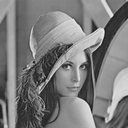
\includegraphics[width = 0.8in]{128.png} $\quad$ and $\bs y = $ 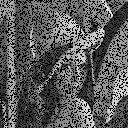
\includegraphics[width=0.8in]{0.png}
\item Then attempt to reconstruct $\bs x$ from $\bs y$
\end{itemize}
\end{frame}

\begin{frame}{Vectorized Signals}
\begin{itemize}%[<+->]
\item Technical Aside: I talk somewhat interchangibly about 2D signals (e.g. images) and 3D signals (e.g. videos)
\item Under the hood, we actually need to store our signals as 1-dimensional vectors
\item Reason: RVM operates on vectors
\item For images, we stack the columns on top of each other to form one long vector in $\mathbb{R}^{hw}$ (\underline{h}eight times \underline{w}idth)
\item For video, we stack the columns in each frame and then stack the \underline{f}rames ($\Rightarrow \bs x \in \mathbb{R}^{hwf}$)
\end{itemize}
\end{frame}

\begin{frame}{Sparse Representations}
\begin{itemize}%[<+->]
\item It is possible to obtain sparse representations for a large variety of signals
\item Common example in signal processing: Transforming sounds from time domain to frequency domain via (Discrete) Fourier Transform 
\item For natural images and image sequences (videos), there are two widely used transforms:
\begin{itemize}
\item Discrete Haar Wavelet Transform
\item Discrete Cosine Transform
\end{itemize}
\item There exist more transforms and probably better ones
\item Ideally, we would like the data to tell us which one to use via some kind of Deep Learning - but this is getting off-topic
\end{itemize}
\end{frame}

\begin{frame}{2D Haar Wavelets}
\begin{itemize}%[<+->]
\item Current prototype uses Haar wavelets at the first scale
\item Very simple: transform essentially consists of taking averages and differences of patches of pixels
\item At scale 1, the individual basis functions have support over $2\times2$ patches
\end{itemize}
\end{frame}

\begin{frame}{2D Haar Wavelets}
\begin{itemize}%[<+->]
\item 2D Haar wavelets at scale 1 can be visualized by 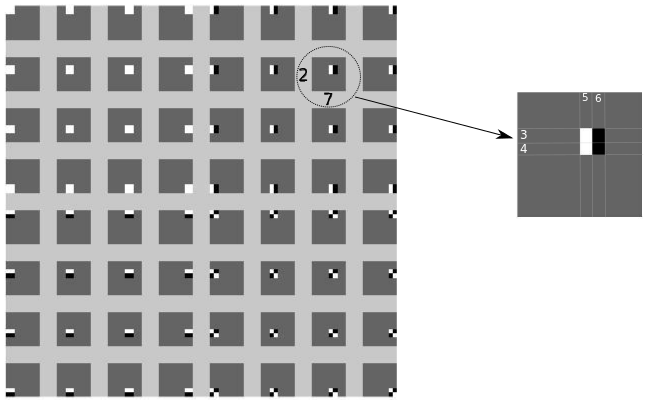
\includegraphics[height=2in]{drawing2.png}
\item White $\equiv +\frac{1}{2}$, black $\equiv-\frac{1}{2}$, dark gray $\equiv0$ 
\item So for example $x_{2,7} \to w_{2,7} = \frac{1}{2}(x_{3,5} - x_{3,6} +  x_{4,5} - x_{4,6})$
\end{itemize}
\end{frame}

\begin{frame}{2D Haar Wavelets: Example}
\begin{itemize}%[<+->]
\item Haar wavelet transform of\\
$\bs x = $ 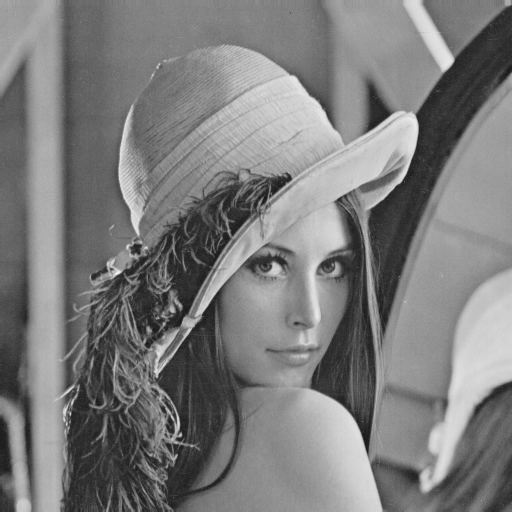
\includegraphics[width=1.5in]{512.png}\, is $\bs w = $ 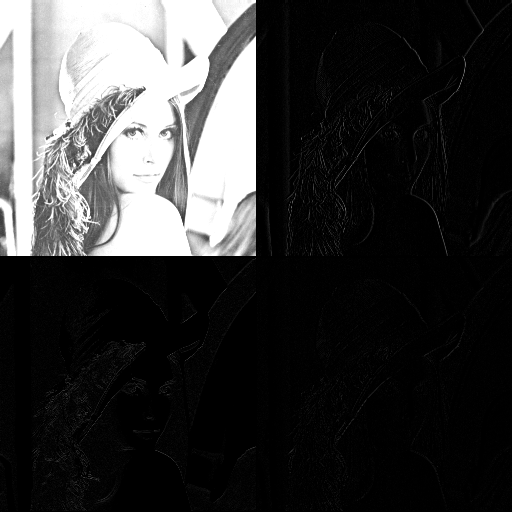
\includegraphics[width=1.5in]{lennaHaar.png}
\item Most entries in $\bs w$ are zero or very close to zero (shown as black) $\Rightarrow \bs w$ is sparse
\end{itemize}
\end{frame}

\begin{frame}{2D Haar Wavelets: Example}
\begin{itemize}%[<+->]
\item Somewhat easier to see what's going on if we invert and translate the colours a little bit:\\
\hspace{1.2in}  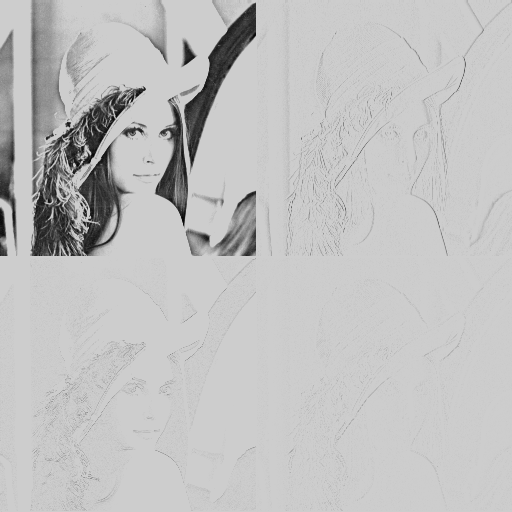
\includegraphics[width=1.5in]{lennaHaarInv.png}
\item Top left is an average of $\bs x$, remaining entries in $\bs w$ are detail coefficients that capture horizontal, verical and diagonal \emph{edges} in $\bs x$ 
\end{itemize}
\end{frame}

\begin{frame}{3D Haar Wavelets}
\begin{itemize}%[<+->]
\item Think of a video as a volume created by stacking the individual frames
\item To take the Haar wavelet transform of a video $\bs x$ we have two approaches:
\begin{itemize}
\item Take the 2D transform of each frame individually $\rightarrow$ process $\bs x$ as a sequence of independent images
\item Use 3D Haar wavelets and process video as a volume $\rightarrow$ exploits continuity between frames
\end{itemize}
\item We used the 3D wavelets approach because it is more general
\item 3D Haar wavelets have support over $2^j\times2^j\times2^j$ blocks (at the $j$th scale)
\end{itemize}
\end{frame}

\begin{frame}{3D Haar Wavelets}
\hspace{0.6in}Demo of Haar wavelet transform of soccer.yuv\\
\hspace{0.8in}$\bs x = $ \hspace{2in}$\bs w = $\\
\movie{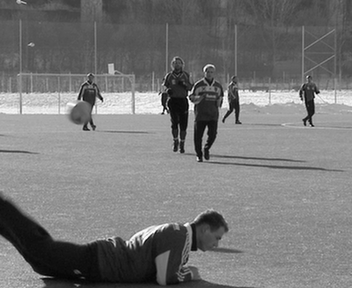
\includegraphics[width=2.2in,height=1.8in]{soccer_raw.png}}{soccer_raw.avi}
\,
\movie{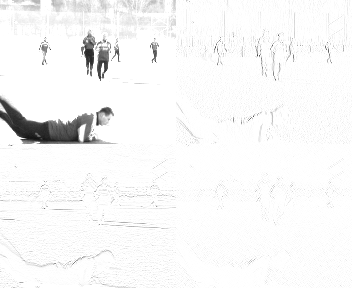
\includegraphics[width=2.2in,height=1.8in]{soccer_haar.png}}{soccer_haar.avi}\\
\hspace{0.4in}(30 frames per second) \hspace{0.8in}(20 frames per second)
\end{frame}

\begin{frame}{Bayesian Compressive Sensing}
\begin{itemize}%[<+->]
\item Recall the goal of Compressive Sensing: Find sparsest solution to $\Phi\bs w = \bs y$ 
\item We mentioned deterministic methods ($L_1$ minimization)
\item But we will use a probabilistic method by treating it as a Machine Learning problem
\item Specifically, we use the RVM to do a regression:
\begin{enumerate}
\item Input a \emph{target vector} $\bs y \in \mathbb{R}^M$
\item Input a \emph{design matrix} $\Phi \in \mathbb{R}^{M\times N}$
\item The RVM outputs a \emph{sparse} coefficients vector $\bs w^* \in \mathbb{R}^N$
\end{enumerate}
\end{itemize}
\end{frame}

\begin{frame}{Bayesian Compressive Sensing}
\begin{itemize}
\item More specifically, RVM gives us a \emph{posterior distribution} for $\bs w^*$: $\bs w^*|\,\mbox{data} \sim \mathcal{N}(\bs\mu,\Sigma)$ 
\item The \emph{posterior mean} $\bs\mu$ is usually very sparse
\item Reconstruct the original signal as $\bs x^* = \Psi\bs\mu$
\item Even better: we can use $\Sigma$ to get error bars in our reconstruction
\item We can use error bars to create a cascade of reconstructions and boost the quality
\item Focus for next couple of days
\end{itemize}
\end{frame}


\begin{frame}{The Relevance Vector Machine: Theory}
\begin{itemize}%[<+->]
\item For our purposes, it is okay to treat the RVM as a ``black box'' 
\item However, if interested in theory:
\item The RVM \cite{tipping2001} is a Bayesian Machine Learning algorithm
\item It was developed by Mike Tipping\cite{tipping2001} and later improved upon by him and Anita Faul\cite{tipping2003}
\end{itemize}
\end{frame}

\begin{frame}{RVM Theory}
\begin{itemize}
\item It models the data as $p(y_i|\,\bs x, \Phi) = \mathcal{N}(y_i|\,\bs w^T \bs \phi(x_i),\sigma^2)$ 
\item Bayesian, so put a prior on $\bs w$: $p(\bs w) = \prod_{j=1}^N \mathcal{N}(w_i|\,0,\alpha_j^{-1})$
\item Use training data (observations) to obtain a posterior for $\bs w$: $p(\bs w) = \mathcal{N}(\bs w|\,\bs\mu,\Sigma)$
\item During training, many $\alpha_j$ become infinite $\Rightarrow w_j = 0$ with infinite precision
\item Thus $\bs w$ is \emph{sparse}
\end{itemize}
\end{frame}

\begin{frame}{Looking Ahead}
\begin{itemize}
\item Progress so far:
\begin{itemize}
\item Implemented a working prototype
\item Use Haar Wavelet transform
\item Got some initial results
\end{itemize}
\item Still to do:
\begin{itemize}
\item Multi-scale Cascade of RVMs
\item Try more Basis Functions, in particular the Discrete Cosine Transform
\item Study: When does it work well, when not?
\item Lit review: How does it compare to other existing methods?
\item How can it be improved?
\end{itemize}
\end{itemize}
\end{frame}

\begin{frame}{Outro}
\hspace{2in}Questions?
\end{frame}

\begin{frame}{More demos}
\hspace{1in} Flickering lines (60\% missing data)\\
\hspace{0.8in}  $\bs y = $ \hspace{2in} $\bs x^* = $\\
\movie{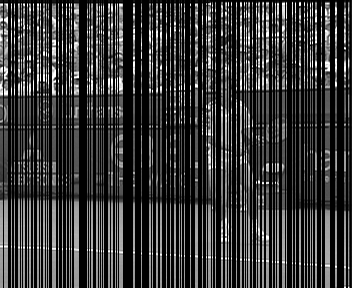
\includegraphics[widht=2.2in,height=1.8in]{stefan_corr.png}}{stefan_corr.avi}
\,
\movie{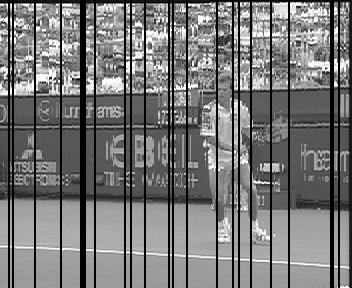
\includegraphics[widht=2.2in,height=1.8in]{stefan_rec.png}}{stefan_rec.avi}
\end{frame}

\begin{frame}{More demos}
\hspace{1in} Uniform noise (60\% missing data)\\
\hspace{0.8in}  $\bs y = $ \hspace{2in} $\bs x^* = $\\
\movie{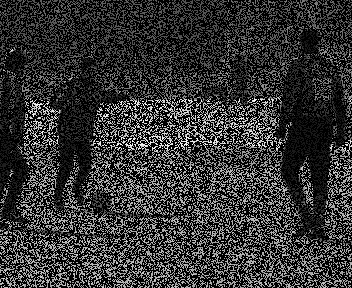
\includegraphics[widht=2.2in,height=1.8in]{soccer_corr.png}}{soccer_corr.avi}
\,
\movie{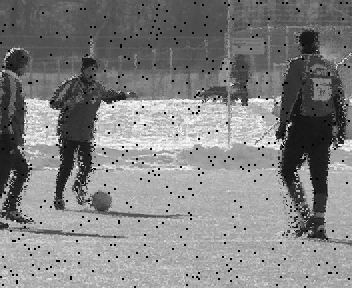
\includegraphics[widht=2.2in,height=1.8in]{soccer_rec.png}}{soccer_rec.avi}
\end{frame}

\begin{frame}{Selected References}
\bibliographystyle{elsarticle-num}
%\bibliographystyle{apa}
\bibliography{referencesRVM.bib}
\end{frame}

\end{document}
